%In Figure 2~\ref{process} the three steps of the conduction phase. As can be seen, in Step 1, we identified primary studies in the digital libraries. The digital libraries Scopus has returned more primary studies than the others(262), i.e., IEEE, ACM and Springer have returned 215, 202 and 127, respectively. Possibly, this came about because this digital library indexes studies of others libraries, such as IEEE and Springer. Summing up, we have gotten 802 primary studies in the Step 1. In the Step 2 we have selected the primary studies by means of reading the titles and abstracts and the application of the inclusion and exclusion criteria. As a result, we have gotten a total of 124 primary studies that were read entirely, so the upshot obtained in the Step 3 were 62. Among these 62 primary studies we have identified 18 mining techniques for crosscutting concern. Therefore, each included primary study was assigned to one or more techniques.
%
%\begin{figure}[!h]
%\centering
%  % Requires \usepackage{graphicx}
%  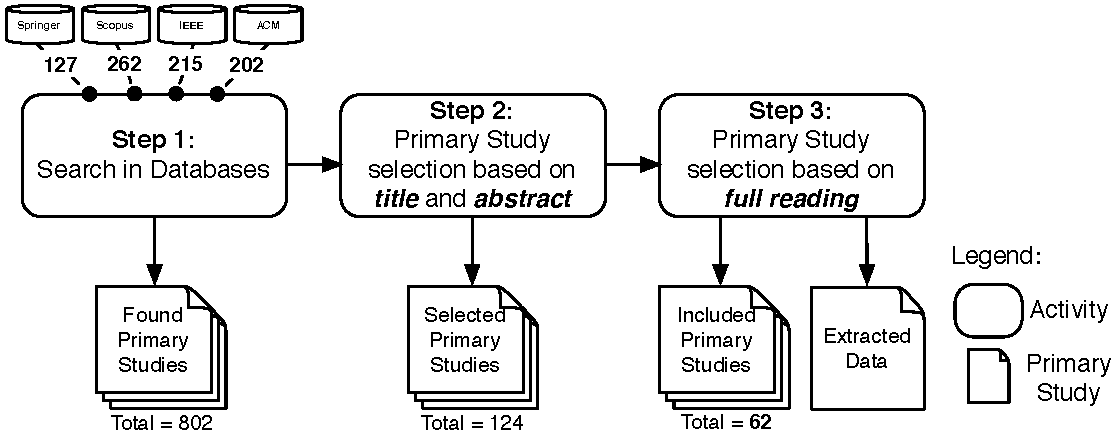
\includegraphics[scale=0.4]{figuras/process_conducted}
%\caption{Papers retrieved from each electronic database, total of candidate studies and the final set.}
%\label{process}
%\end{figure} 

Firstly we applied the search string given in Figure~\ref{search_string} in some digital libraries. An overview of results acquired from these digital libraries is depicted in Table~\ref{result_digital}.
\begin{table}[!h]
\centering
\caption{Overview of search results.}
\begin{tabular}{p{\dimexpr.25\textwidth}p{\dimexpr.16\textwidth-4\tabcolsep}}
\hline 
Digital Libraries & Number\tabularnewline
\hline 
Scopus & 150
\\
ACM & 51
\\ 
Engeneering Village & 30
\\
Web of Science & 17
\\
IEEE & 11
\\
Total & 259
\\
Candidates & 82
\\
Final set & 30\tabularnewline
\hline 
\end{tabular}
\label{result_digital}
\end{table} 
As can be seen in this table, the digital libraries Scopus returned more primary studies than the others (150), ACM, Engeneering Village, Web of Science and IEEE returned 51, 30, 17 and 11, respectively. Possibly, this occurred because Scopus indexes studies of others libraries, such as IEEE and ACM. Summarizing, we obtained 259 primary studies. After performing automatic search, we excluded the duplicate publications. If a primary study was found in more than once, we selected the most recent and detailed version of the paper. Afterwards, we selected the primary studies by reading the titles and abstracts and the application of the inclusion and exclusion criteria. At this stage, we also narrowed down the categories of publications to some extent by excluding non-peer reviewed publications, in order to ensure a level of quality as well as to avoid redundancy in contributions. As a result, we acquired a total of 82 primary studies that were read entirely, so the upshot obtained were 30 studies. A total of 229 studies were excluded either due to their limited relevance or meeting one of the other exclusion criterions.

We applied the classification schemes proposed by Petersen et al.~\cite{Petersen:2008:SMS:2227115.2227123} and classified the publications into categories from three perspectives, as follows: (\textit{i}) focus area, (\textit{ii}) contribution type and (\textit{iii}) research type. We chose this classification scheme because it is highly used in secondary study, i.e., papers which describe systematic review~\cite{Durelli:2013:SRM:2480362.2480567}.% and systematic mapping~\cite{Mehmood:2013:AMC:2400747.2401009}. %Although, this classification schemes has been proposed to be applied during a systematic mapping, we claim that it can be used during the systematic review process as well. 
 Thus, the aforementioned categories were adapted to our systematic study. We identified four focus areas, five contribution types and five research types. Notice that the research types reflects the research approach used in the primary study. We used and adapted the scheme proposed by Wieringa et al~\cite{Wieringa:2005:REP:1107677.1107683} herein. The resultant classification schemes are as follows:

\begin{enumerate}

\item Focus Areas: 

\begin{enumerate}

\item Software Modernization: This focus area is related to primary studies which describe approaches that use ADM to fully modernize legacy systems either to another platform  or architecture;

\item Business Knowledge Extraction: Describes primaries studies which address process, method or approach to extract business process of a legacy system;

\item Concern Extraction: Describes primaries studies which address process, method or approach to extract crosscutting concerns (CC) of a legacy system. Examples of CC are persistence, security and distribution;

\item Extension of ADM's Metamodels: This focus area represents primary studies which report an approach, method or process to extend one of the ADM's metamodels;

\item Applicability: This category includes papers that mainly focus on reporting evidence related to applying ADM and its metamodels in practice. In other words, papers which enable researchers and practitioners to get a better understanding and utilization of ADM and its metamodels.

\end{enumerate}

\item Contribution Type:

\begin{enumerate}

\item Tool: Refers to primary studies that focus on providing tools to support the modernization of legacy system by using ADM; 

\item Process: Refers to papers which describe processes to assist the modernization of legacy system by means of ADM;

\item Model Transformation: Refers papers that describe the use of language transformation such as Query/Views/Transformations (QVT)\footnote{http://www.omg.org/spec/QVT/1.1/} or ATL Transformation Language (ATL)\footnote{www.eclipse.org/atl/} to realize transformation among the ADM's metamodels;

\item Metamodel: Describes primary studies which create or extend the ADM's metamodels to deal with a specific problem, for instance, providing a KDM light-weight extension in order to either represent the aspect oriented paradigm or supports a component-oriented decomposition;

\item Metrics: Describes papers that focus on proposing or applying metrics to effectiveness of ADM and its metamodels.

\end{enumerate}

\item Research Type:

\begin{enumerate}

\item Validation research: Validation research is conducted in a systematic way and may present any of these: prototypes, math analysis, etc;

\item Evaluation research: In contrast to validation research, evaluation research aims at examining a solution that has already been practically applied. It investigates the practical implementation of solution and usually presents results using field studies, experiments, or case studies, etc;

\item Conceptual proposal: A conceptual proposal presents an arrangement to perceive things that already exist, in a novel way;

\item Experience paper: An experience paper reports on personal experience of the author from one or more real life projects;

\item Opinion paper:  Opinion papers report on personal opinion of the author on suitability or unsuitability of a specific technique or tool.

\end{enumerate}

\end{enumerate}